% !TeX program = xelatex
% !TeX encoding = utf8
% !TeX root = FuVar.tex

%% TODO: publish to CTAN
\documentclass[twocolumn, margin=small]{tex/hsrzf}

%%%%%%%%%%%%%%%%%%%%%%%%%%%%%%%%%%%%%%%%%%%%%%%%%%%
% Packages

%% TODO: publish to CTAN
\usepackage{tex/hsrstud}

%% Language configuration
\usepackage{polyglossia}
\setdefaultlanguage{english}

%% License configuration
\usepackage[
    type={CC},
    modifier={by-nc-sa},
    version={4.0},
    lang={english},
]{doclicense}

%% Math
\usepackage{amsmath}
\usepackage{amsthm}
\usepackage{mathtools}

%% Layout
\usepackage{enumitem}
\usepackage{booktabs}
\usepackage{footmisc}

%% Nice drwaings
\usepackage{tikz}

%%%%%%%%%%%%%%%%%%%%%%%%%%%%%%%%%%%%%%%%%%%%%%%%%%%
% Metadata

\course{Elektrotechnik}
\module{FuVar}
\semester{Spring Semseter 2021}

\authoremail{naoki.pross@ost.ch}
\author{\textsl{Naoki Pross} -- \texttt{\theauthoremail}}

\title{Notes of ``Funktionen mehrerer Variablen''}
\date{\thesemester}

%%%%%%%%%%%%%%%%%%%%%%%%%%%%%%%%%%%%%%%%%%%%%%%%%%%
% Macros and settings

\setlength{\droptitle}{-1cm}

%% Theorems
\newtheoremstyle{fuvarzf} % name of the style to be used
  {\topsep}
  {\topsep}
  {}
  {0pt}
  {\bfseries}
  {.}
  { }
  { }

\theoremstyle{fuvarzf}
\newtheorem{theorem}{Theorem}
\newtheorem{method}{Method}
\newtheorem{application}{Application}
\newtheorem{definition}{Definition}
\newtheorem{remark}{Remark}
\newtheorem{note}{Note}

\DeclareMathOperator{\tr}{\mathrm{tr}}

\setlist[description]{
  format = { \normalfont\itshape }
}

%%%%%%%%%%%%%%%%%%%%%%%%%%%%%%%%%%%%%%%%%%%%%%%%%%%
% Document

\begin{document}

\maketitle
% \tableofcontents

\section{Preface}

These are just my personal notes of the \themodule{} course, and definitively
not a rigorously constructed mathematical text.

\section{Derivatives of vector valued scalar functions}

\begin{definition}[Partial derivative]
  A vector valued function \(f: \mathbb{R}^m\to\mathbb{R}\), with
  \(\vec{v}\in\mathbb{R}^m\), has a partial derivative with respect to \(v_i\)
  defined as
  \[
    \partial_{v_i} f(\vec{v})
      % = f_{v_i}(\vec{v})
      = \frac{\partial f}{\partial v_i}
      = \lim_{h\to 0} \frac{f(\vec{v} + h\vec{e}_i) - f(\vec{v})}{h}
  \]
\end{definition}

\begin{theorem}(Schwarz's theorem, symmetry of partial derivatives)
  Under some generally satisfied conditions (continuity of \(n\)-th order
  partial derivatives) Schwarz's theorem states that it is possible to swap
  the order of differentiation.
  \[
    \partial_x \partial_y f(x,y) = \partial_y \partial_x f(x,y)
  \]
\end{theorem}

\begin{application}[Find the slope of an implicit curve]
  Let \(f(x,y) = 0\) be an implicit curve. Its slope at any point where
  \(\partial_y f \neq 0\) is \(m = - \partial_x f / \partial_y f\)
\end{application}

\begin{definition}[Total differential]
  The total differential \(df\) of \(f:\mathbb{R}^m\to\mathbb{R}\) is
  \[
    df = \sum_{i=1}^m \partial_{x_i} f\cdot dx .
  \]
  That reads, the \emph{total} change is the sum of the change in each
  direction. This implies
  \[
    \frac{df}{dx_k} = \frac{\partial f}{\partial x_k} + 
      \sum_{i \in \{1 \leq i \leq m : i \neq k\}}
      \frac{\partial f}{\partial x_i} \cdot \frac{dx_i}{dx_k} ,
  \]
  i.e. the change in direction \(x_k\) is how \(f\) changes in \(x_k\)
  (ignoring other directions) plus, how \(f\) changes with respect to each
  other variable \(x_i\) times how they (\(x_i\)) change with respect to \(x_k\).
\end{definition}

\begin{application}[Linearization]
  A function \(f: \mathbb{R}^m\to\mathbb{R}\) has a linearization \(g\) at
  \(\vec{x}_0\) given by
  \[
    g(\vec{x}) = f(\vec{x}_0) 
      + \sum_{i=1}^m \partial_{x_i} f(\vec{x}_0)(x_i - x_{i,0}) ,
  \]
  if all partial derivatives are defined at \(\vec{x}_0\). With the gradient
  (defined below) \(g(\vec{x}) = f(\vec{x}_0) + \grad f(\vec{x}_0) \dotp
  (\vec{x} - \vec{x}_0)\).
\end{application}

\begin{application}[Propagation of uncertanty]
  Given a measurement of \(m\) values in a vector \(\vec{x}\in\mathbb{R}^m\)
  with values given in the form \(x_i = \bar{x}_i \pm \sigma_{x_i}\), a linear
  approximation of the error of a dependent variable \(y = f(\vec{x})\) is
  computed with
  \[
    y = \bar{y} \pm \sigma_y \approx f(\bar{\vec{x}})
      \pm \sqrt{\sum_{i=1}^m \left(
        \partial_{x_i} f(\bar{\vec{x}}) \sigma_{x_i}\right)^2}
  \]
\end{application}

\begin{definition}[Gradient vector]
  The \emph{gradient} of a function \(f(\vec{x}), \vec{x}\in\mathbb{R}^m\) is a
  column vector\footnote{In matrix notation it is also often defined as row
  vector to avoid having to do some transpositions in the Jacobian matrix and
  dot products in directional derivatives} containing the partial derivatives
  in each direction.
  \[
    \grad f (\vec{x}) = \sum_{i=1}^m \partial_{x_i} f(\vec{x}) \vec{e}_i
      = \begin{pmatrix}
        \partial_{x_1} f(\vec{x}) \\
        \vdots \\
        \partial_{x_m} f(\vec{x}) \\
      \end{pmatrix}
  \]
\end{definition}

\begin{theorem}
  The gradient vector always points towards \emph{the direction of steepest
  ascent}, and thus is always perpendicular to contour lines.
\end{theorem}

\begin{definition}[Directional derivative]
  A function \(f(\vec{x})\) has a directional derivative in direction
  \(\vec{v}\) (with \(|\vec{v}|=1\)) of
  \[
    \frac{\partial f}{\partial\vec{v}} 
      = \nabla_\vec{v} f = \vec{v} \dotp \grad f
      = \sum_{i=1}^m v_i \partial_{x_i} f
  \]
\end{definition}

\begin{definition}[Jacobian Matrix]
  The \emph{Jacobian} \(\mx{J}_f\) (sometimes written as
  \(\frac{\partial(f_1,\ldots f_m)}{\partial(x_1,\ldots,x_n)}\)) of a function
  \(\vec{f}: \mathbb{R}^m \to \mathbb{R}^n\) is a matrix
  \(\in\mathbb{R}^{m\times n}\) whose entry at the \(i\)-th row and \(j\)-th
  column is given by \((\mx{J}_f)_{i,j} = \partial_{x_j} f_i\), so
  \[
    \mx{J}_f = \begin{pmatrix}
      \partial_{x_1} f_1 & \cdots & \partial_{x_m} f_1 \\
      \vdots & \ddots & \vdots \\
      \partial_{x_1} f_n & \cdots & \partial_{x_m} f_n \\
    \end{pmatrix}
    = \begin{pmatrix}
      (\grad f_1)^t \\
      \vdots \\
      (\grad f_m)^t \\
    \end{pmatrix}
  \]
\end{definition}

\begin{remark}
  In the scalar case (\(n = 1\)) the Jacobian matrix is the transpose of the
  gradient vector.
\end{remark}

\begin{definition}[Hessian matrix]
  Given a function \(f: \mathbb{R}^m \to \mathbb{R}\), the square matrix whose
  entry at the \(i\)-th row and \(j\)-th column is the second derivative of
  \(f\) first with respect to \(x_j\) and then to \(x_i\) is known as the
  \emph{Hessian} matrix.
  \(
    \left(\mx{H}_f\right)_{i,j} = \partial_{x_i}\partial_{x_j} f
  \)
  or
  \[
    \mx{H}_f = \begin{pmatrix}
      \partial_{x_1}\partial_{x_1} f & \cdots & \partial_{x_1}\partial_{x_m} f \\
      \vdots & \ddots & \vdots \\
      \partial_{x_m}\partial_{x_1} f & \cdots & \partial_{x_m}\partial_{x_m} f \\
    \end{pmatrix}
  \]
  Because (almost always) the order of differentiation
  does not matter, it is a symmetric matrix.
\end{definition}


\section{Methods for maximization and minimization problems}

\subsection{Analytical methods}

\begin{method}[Find stationary points]
  Given a function \(f: D \subseteq \mathbb{R}^m \to \mathbb{R}\), to
  find its maxima and minima we shall consider the points
  \begin{itemize}
    \item that are on the boundary\footnote{If it belongs to \(f\).
      \label{ftn:boundary}} of the domain \(\partial D\),
    \item where the gradient \(\grad f\) is not defined,
    \item that are stationary, i.e. where \(\grad f = \vec{0}\).
  \end{itemize}
\end{method}

\begin{method}[Determine the type of stationary point for 2 dimensions]
  Given a scalar function of two variables \(f(x,y)\) and a stationary point
  \(\vec{x}_s\) (where \(\grad f(\vec{x}_s) = \vec{0}\)), we define the
  \emph{discriminant}
  \[
    \Delta = \partial_x^2 f \partial_y^2 f - \partial_y \partial_x f
  \]
  \begin{itemize}
    \item if \(\Delta > 0\) then \(\vec{x}_s\) is an extrema, if \(\partial_x^2
      f(\vec{x}_s) < 0\) it is a maximum, whereas if \(\partial_x^2
      f(\vec{x}_s) > 0\) it is a minimum;

    \item if \(\Delta < 0\) then \(\vec{x}_s\) is a saddle point;

    \item if \(\Delta = 0\) we need to analyze further.
  \end{itemize}
\end{method}

\begin{remark}
  The previous method is obtained by studying the second directional derivative
  \(\nabla_\vec{v}\nabla_\vec{v} f\) at the stationary point in direction of a
  vector \(\vec{v} = \vec{e}_1\cos(\alpha) + \vec{e}_2\sin(\alpha)\).
\end{remark}

\begin{method}[Determine the type of stationary point in higher dimensions]
  Given a scalar function of multiple variables \(f(\vec{x})\) and a stationary
  point \(\vec{x}_s\) (\(\grad f(\vec{x}_s) = \vec{0}\)), we compute the
  Hessian matrix \(\mx{H}_f(\vec{x}_s)\) and its eigenvalues \(\lambda_1,
  \ldots, \lambda_m\), then
  \begin{itemize}
    \item if all \(\lambda_i > 0\), the point is a minimum;
    \item if all \(\lambda_i < 0\), the point is a maximum;
    \item if there are both positive and negative eigenvalues,
      it is a saddle point.
  \end{itemize}
  In the other cases, when there are \(\lambda_i \leq 0\) and/or \(\lambda_i
  \geq 0\) further analysis is required.
\end{method}

\begin{remark}
  Recall that to compute the eigenvalues of a matrix, one must solve the
  equation \((\mx{H} - \lambda\mx{I})\vec{x} = \vec{0}\). Which can be done
  by solving the characteristic polynomial \(\det\left(\mx{H} -
  \lambda\mx{I}\right) = 0\) to obtain \(\dim(\mx{H})\) \(\lambda_i\), which
  when plugged back in result in a overdetermined system of equations.
\end{remark}

\begin{method}[Quickly find the eigenvalues of a \(2\times 2\) matrix]
  This is a nice trick. For a square matrix \(\mx{H}\), let
  \[
    m = \frac{1}{2}\tr \mx{H} = \frac{a + d}{2} ,
    \quad
    p = \det\mx{H} = ad - bc ,
  \]
  then \(\lambda_{1,2} = m \pm \sqrt{m^2 - p}\).
\end{method}

\begin{method}[Search for a constrained extremum in 2 dimensions]
  Let \(n(x,y) = 0\) be a constraint in the search of the extrema of a function
  \(f: D \subseteq \mathbb{R}^2 \to \mathbb{R}\). To find the extrema we look for
  points
  \begin{itemize}
    \item on the boundary\footref{ftn:boundary} \(\vec{u} \in \partial D\)
      where \(n(\vec{u}) = 0\);

    \item \(\vec{u}\) where the gradient either does not exist or is
      \(\vec{0}\), and satisfy \(n(\vec{u}) = 0\);

    \item that solve the system of equations
      \[
        \begin{cases}
          \partial_x f(\vec{u}) \cdot \partial_y n(\vec{u})
            = \partial_y f(\vec{u}) \cdot \partial_x n(\vec{u}) \\
          n(\vec{u}) = 0
        \end{cases}
      \]
  \end{itemize}
\end{method}

\begin{figure}
  \centering
  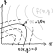
\includegraphics{img/lagrange-multipliers}
  \caption{
    Intuition for the method of Lagrange multipliers.  Extrema of a constrained
    function are where \(\grad f\) is proportional to \(\grad n\).
  }
\end{figure}

\begin{method}[%
    Search for a constrained extremum in higher dimensions,
    method of Lagrange multipliers]
  We wish to find the extrema of \(f: D \subseteq \mathbb{R}^m \to \mathbb{R}\)
  under \(k < m\) constraints \(n_1 = 0, \cdots, n_k = 0\). To find the extrema 
  we consider the following points:
  \begin{itemize}
    \item Points on the boundary\footref{ftn:boundary} \(\vec{u} \in \partial D\) that satisfy
      \(n_i(\vec{u}) = 0\) for all \(1 \leq i \leq k\), 

    \item Points \(\vec{u} \in D\) where either
      \begin{itemize}
        \item any of \(\grad f, \grad n_1, \ldots, \grad n_k\) do not exist, or
        \item \(\grad n_1, \ldots, \grad n_k\) are linearly \emph{dependent},
      \end{itemize}
      and that satisfy \(0 = n_1(\vec{u}) = \ldots = n_k(\vec{u})\).

    \item Points that solve the system of \(m+k\) equations
      \[
        \begin{dcases}
          \grad f(\vec{u}) = \sum_{i = 1}^k \lambda_i \grad n_i(\vec{u})
            & (m\text{-dimensional}) \\
          n_i(\vec{u}) = 0  & \text{ for } 1 \leq i \leq k
        \end{dcases}
      \]
      The \(\lambda\) values are known as \emph{Lagrange multipliers}.
  \end{itemize}
  The calculation of the last point can be written more compactly by defining
  the \emph{Lagrangian}
  \[
    \mathcal{L}(\vec{u}, \vec{\lambda}) 
    = f(\vec{u}) - \sum_{i = 0}^k \lambda_i n_i(\vec{u}),
  \]
  where \(\vec{\lambda} = \lambda_1, \ldots, \lambda_k\) and then solving
  the \(m+k\) dimensional equation \(\grad \mathcal{L}(\vec{u},
  \vec{\lambda}) = \vec{0}\) (this is generally used in numerical
  computations and not very useful by hand).
\end{method}

\subsection{Numerical methods}

\begin{method}[Newton's method]
  For a function \(f:\mathbb{R}^m\to\mathbb{R}\) we wish to numerically find
  its stationary points (where \(\grad f = \vec{0}\)).
  \begin{enumerate}
    \item Pick a starting point \(\vec{x}_0\).
    \item Set the linearisation\footnote{The gradient becomes a hessian matrix.}
      of \(\grad f\) at \(\vec{x}_k\) to zero and
      solve for \(\vec{x}_{k+1}\).
      \begin{gather*}
        \grad f(\vec{x}_k) + \mx{H}_f (\vec{x}_k)
          (\vec{x}_{k+1} - \vec{x}_k) = \vec{0} \\
          \vec{x}_{k+1} = \vec{x}_k - \mx{H}_f^{-1} (\vec{x}_k) \grad f(\vec{x}_k)
      \end{gather*}
    \item Repeat the last step until the magnitude of the error
      \(|\vec{\epsilon}| = |\mx{H}_f^{-1} (\vec{x}_k) \grad f(\vec{x}_k)|\) is
      sufficiently small.
  \end{enumerate}
\end{method}

\begin{method}[Gradient ascent / descent]
  Given \(f:\mathbb{R}^m\to\mathbb{R}\) we wish to numerically find
  the stationary points (where \(\grad f = \vec{0}\)).
  \begin{enumerate}
    \item Define an arbitrarily small length \(\eta\) and a starting point
      \(\vec{x}_0\)
    \item Compute \(\vec{v} = \pm\grad f(\vec{x}_k)\) (positive for ascent,
      negative for descent), then \(\vec{x}_{k+1} = \vec{x}_k + \eta\vec{v}\)
      if the rate of change \(\epsilon\) is acceptable (\(\epsilon = |\grad
      f(\vec{x}_{k+1})| > 0\)) else recompute \(\vec{v} := \pm \grad
      f(\vec{x}_{k+1})\).
    \item Stop when the rate of change \(\epsilon\) stays small enough for many
      iterations.
  \end{enumerate}
\end{method}

\section{Integration of vector valued scalar functions}

\begin{figure}
  \centering
  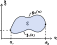
\includegraphics{img/double-integral}
  \caption{
    Double integral.
    \label{fig:double-integral}
  }
\end{figure}

\begin{theorem}[Change the order of integration for double integrals] For a
  double integral over a region \(S\) (see Fig.  \ref{fig:double-integral}) we
  need to compute
  \[
    \iint_S f(x,y) \,ds =
      \int\limits_{x_1}^{x_2} \int\limits_{y_1(x)}^{y_2(x)} f(x,y) \,dydx .
  \]
  If \(y_1(x)\) and \(y_2(x)\) are bijective we can swap the order of
  integration by finding the inverse functions \(x_1(y)\) and \(x_2(y)\). If
  they are not bijective (like in Fig. \ref{fig:double-integral}), the region
  must be split into smaller parts. If the region is a rectangle it is always
  possible to change the order of integration.
\end{theorem}

\begin{theorem}[Transformation of coordinates in 2 dimensions]
  \label{thm:transform-coords}
  Given two ``nice'' functions \(x(u,v)\) and \(y(u,v)\), that means are a
  bijection from \(S\) to \(S'\) with continuous partial derivatives and
  nonzero Jacobian determinant \(|\mx{J}| = \partial_u x \partial_v y -
  \partial_v x \partial_u y\), which transform the coordinate system. Then
  \[
    \iint_S f(x,y) \,ds = \iint_{S'} f(x(u,v), y(u,v)) |\mx{J}| \,ds .
  \]
\end{theorem}

\begin{theorem}[Transformation of coordinates]
  The generalization of theorem \ref{thm:transform-coords} is quite simple.
  For an \(m\)-integral of a function \(f:\mathbb{R}^m\to\mathbb{R}\) over a
  region \(B\), we let \(\vec{g}(\vec{u})\) be ``nice'' functions that
  transform the coordinate system. Then as before
  \[
    \int_B f(\vec{r}) \,ds = \int_{B'} f(\vec{g}(\vec{u})) |\mx{J}_\vec{g}| \,ds .
  \]
\end{theorem}

\begin{application}[Physics]
  Given the mass \(m\) and density function \(\rho\) of an object,
  its \emph{center of mass} is calculated with
  \[
    \vec{x}_c = \frac{1}{m}\int_V \rho(\vec{r})\vec{r} \,dv
      \stackrel{\rho\text{ const.}}{=} \frac{1}{V} \int_V \vec{r}\,dv .
  \]
  The (scalar) \emph{moment of inertia} \(J\) of an object is given by
  \[
    J = \int_V \rho(\vec{r}) r^2 \,dv .
  \]
  % and similarly the \emph{area moment of inertia} \(I\)
\end{application}

\section{Parametric curves, line and surface integrals}

\begin{definition}[Parametric curve]
  A parametric curve is a vector function \(\mathcal{C} : \mathbb{R} \to W
  \subseteq \mathbb{R}^n, t \mapsto \vec{f}(t)\), that takes a parameter \(t\).
\end{definition}

\begin{theorem}[Derivative of a curve]
  The derivative of a curve is
  \begin{align*}
    \vec{f}'(t) &= \lim_{h\to 0} \frac{\vec{f}(t + h) - \vec{f}(t)}{h} \\
    &= \sum_{i=0}^n \left(\lim_{h\to 0} \frac{f_i(t+h) - f_i(t)}{h}\right) \vec{e}_i \\
    &= \sum_{i=0}^n \frac{df_i}{dt}\vec{e}_i
    = \left(\frac{df_1}{dt}, \ldots, \frac{df_m}{dt}\right)^t .
  \end{align*}
\end{theorem}

% \begin{figure}
%   \centering
%   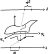
\includegraphics{img/multivariable-chain-rule}
%   \caption{
%     Multivariable chain rule.
%   }
% \end{figure}

\begin{theorem}[Multivariable chain rule]
  Let \(\vec{x}: \mathbb{R} \to \mathbb{R}^m\) and \(f: \mathbb{R}^m \to
  \mathbb{R}\), so that \(f\circ\vec{x}: \mathbb{R} \to \mathbb{R}\), then
  the multivariable chain rule states:
  \[
    \frac{d}{dt}f(\vec{x}(t)) = \grad f (\vec{x}(t)) \dotp \vec{x}'(t)
      = \nabla_{\vec{x}'(t)} f(\vec{x}(t)) .
  \]
\end{theorem}

\begin{theorem}[Signed area enclosed by a planar parametric curve]
  A planar (2D) parametric curve \((x(t), y(t))^t\) with \(t\in[r,s]\) that does
  not intersect itself encloses a surface with area
  \[
    A = \int_r^s x'(t)y(t) \,dt
      = \int_r^s x(t)y'(t) \,dt .
  \]
\end{theorem}

\begin{definition}[Line integral in a scalar field]
  Let \(\mathcal{C}:[a,b]\to\mathbb{R}^n, t \mapsto \vec{r}(t)\) be a
  parametric curve. The \emph{line integral} in a field \(f(\vec{r})\) is the
  integral of the signed area under the curve traced in \(\mathbb{R}^n\), and
  is computed with
  \[
    \int_\mathcal{C} f(\vec{r}) \,d\ell 
    = \int_\mathcal{C} f(\vec{r}) \,|d\vec{r}|
    = \int_a^b f(\vec{r}(t)) |\vec{r}'(t)| \, dt .
  \]
\end{definition}

\begin{application}[Length of a parametric curve]
  By computing the line integral of the function \(1(\vec{r})\) we get the
  length of the parametric curve \(\mathcal{C}:[a,b]\to\mathbb{R}^n\).
  \[
    \int_\mathcal{C}d\ell 
    = \int_\mathcal{C} |d\vec{r}|
    = \int_a^b \sqrt{\sum_{i=1}^n x'_i(t)^2} \,dt
  \]
  The special case with the scalar function \(f(x)\) results in
  \(\int_a^b\sqrt{1+f'(x)^2}\,dx\).
\end{application}

\begin{figure}
  \centering
  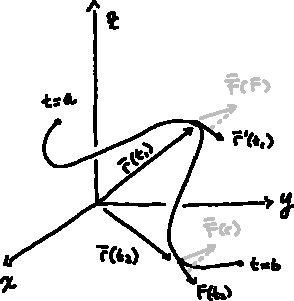
\includegraphics{img/line-integral}
  \caption{
    Line integral in a vector field.
  }
\end{figure}

\begin{definition}[Line integral in a vector field]
  The line integral in a vector field \(\vec{F}(\vec{r})\) is the ``sum'' of
  the projections of the field's vectors on the tangent of the parametric curve
  \(\mathcal{C}\).
  \[
    \int_\mathcal{C} \vec{F}(\vec{r})\dotp d\vec{r}
    = \int_a^b \vec{F}(\vec{r}(t))\dotp \vec{r}'(t) \,dt
  \]
\end{definition}

\begin{theorem}[Line integral in the opposite direction]
  By integrating while moving backwards (\(-t\)) on the parametric curve gives
  \[
    \int_{-\mathcal{C}} \vec{F}(\vec{r})\dotp d\vec{r}
    = -\int_{\mathcal{C}} \vec{F}(\vec{r})\dotp d\vec{r} .
  \]
\end{theorem}

\begin{definition}[Conservative field]
  A vector field is said to be \emph{conservative} the line integral over a
  closed path is zero.
  \[
    \oint_\mathcal{C} \vec{F}(\vec{r})\cdot d\vec{r} = 0
  \]
\end{definition}

\begin{theorem}
  For a twice partially differentiable vector field \(\vec{F}\) in
  \(n\) dimensions without ``holes'', i.e. in which each closed curve can be
  contracted to a point (simply connected open set), the following statements
  are equivalent:
  \begin{itemize}
    \item \(\vec{F}\) is conservative,
    \item \(\vec{F}\) is path-independent,
    \item \(\vec{F}\) is a \emph{gradient field}, i.e. there is a
      function \(\phi\) called \emph{potential} such that \(\vec{F} = \grad
      \phi\),
    \item \(\vec{F}\) satisfies the condition \(\partial_{x_j} F_i =
      \partial_{x_i} F_j\) for all \(i,j \in \{1,2,\ldots,n\}\). In the 2D case
      \(\partial_x F_y = \partial_y F_x\), and in 3D
      \[
        \begin{cases}
          \partial_y F_x = \partial_x F_y \\
          \partial_z F_y = \partial_y F_z \\
          \partial_x F_z = \partial_z F_x \\
        \end{cases}
      \]
  \end{itemize}
\end{theorem}

\begin{theorem}
  In a conservative field \(\vec{F}\) with gradient \(\phi\), using the
  multivariable the chain rule:
  \begin{align*}
    \int_\mathcal{C} \vec{F} \dotp d\vec{r} 
    &= \int_\mathcal{C} \vec{F}(\vec{r}(t)) \dotp \vec{r}'(t) \,dt \\
    &= \int_\mathcal{C} \grad \phi(\vec{r}(t)) \cdot \vec{r}'(t) \,dt \\
    &= \int_\mathcal{C} \frac{d\phi(\vec{r}(t))}{dt}\,dt
    = \phi(\vec{r}(b)) - \phi(\vec{r}(a)) .
  \end{align*}
\end{theorem}

\begin{definition}[Parametric surface]
  A parametric surface is a vector function \(\mathcal{S}: W \subseteq \mathbb{R}^2 \to
  \mathbb{R}^3\).
\end{definition}

\begin{figure}
  \centering
  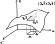
\includegraphics{img/surface-integral}
  \caption{
    Surface integral.
  }
\end{figure}

\begin{theorem}[Area of a parametric surface]
  The area spanned by a parametric surface \(\vec{s}(u,v)\), with continuous
  partial derivatives and that satisfy \(\partial_u \vec{s} \crossp \partial_v
  \vec{s} \neq \vec{0}\), is given by
  \[
    A = \int_\mathcal{S} ds 
      = \iint |\partial_u \vec{s} \crossp \partial_v \vec{s}| \,dudv .
  \]
\end{theorem}

\begin{definition}[Scalar surface integral]
  Let \(f: \mathbb{R}^3 \to \mathbb{R}\) be a function on a parametric surface
  \(\vec{s}: W \subseteq \mathbb{R}^2 \to \mathbb{R}^3\).  The surface integral
  of \(f\) over \(\mathcal{S}\) is
  \[
    \int_\mathcal{S} f \,ds = 
      \iint_W f(\vec{s}(u,v)) \cdot 
        |\partial_u \vec{s} \crossp \partial_v \vec{s}| \,dudv .
  \]
\end{definition}

\begin{table}
  \centering
  \begin{tabular}{l >{\(}l<{\)} >{\(}l<{\)}}
    \toprule
    & \text{Volume } dv & \text{Surface } d\vec{s}\\
    \midrule
    Cartesian & - & dx\,dy     \\
    Polar     & - & rd\,rd\phi \\
    Curvilinear & - & |\mx{J}_f|\,du\,dv \\
    \midrule
    Cartesian   & dx\,dy\,dz                         & \uvec{z}\,dx\,dy     \\
    Cylindrical & r\,dr\,d\phi\,dz                   & \uvec{z}r\,dr\,d\phi \\
                &                                    & \uvec{\phi}\,dr\,dz  \\
                &                                    & \uvec{r}r\,d\phi\,dz \\
    Spherical   & r^2\sin\theta\, dr\,d\theta\,d\phi & 
      \uvec{r}r^2\sin\theta\,d\theta\,d\phi \\
    Curvilinear & |\mx{J}_f|\,du\,dv\,dw & - \\
    \bottomrule
  \end{tabular}
  \caption{Differential elements for integration.}
\end{table}

\section{Vector analysis}

\begin{definition}[Flux]
  In a vector field \(\vec{F}: \mathbb{R}^m \to \mathbb{R}^n\) we define the
  \emph{flux} through a parametric surface \(\mathcal{S}\) as
  \[
    \Phi = \int_\mathcal{S} \vec{F} \dotp d\vec{s} 
      = \int_\mathcal{S} \vec{F} \dotp \uvec{n} \,ds .
  \]
  If \(\mathcal{S}\) is a closed surface we write
  \(
    \mathring{\Phi} = \oint_\mathcal{S} \vec{F} \dotp d\vec{s}
  \).
\end{definition}

If we now take the normalized flux on the surface of an arbitrarily small
volume \(V\) (limit as \(V\to 0\)) we get the \emph{divergence}
\[
  \div \vec{F} = \lim_{V\to 0} \frac{1}{V} \oint_{\partial V} \vec{F}\dotp d\vec{s} .
\]

\begin{theorem}[Formula for divergence]
  Let \(\vec{F}: \mathbb{R}^m \to \mathbb{R}^m\) be a vector field.
  The divergence of \(\vec{F} = (F_{x_1},\ldots, F_{x_m})^t\) is
  \[
    \div\vec{F} = \sum_{i = 1}^m \partial_{x_i} F_{x_i} ,
  \]
  as suggested by the (ab)use of the dot product notation.
\end{theorem}

\begin{theorem}[Divergence theorem, Gauss's theorem]
  Because the flux on the boundary \(\partial V\) of a volume \(V\) contains
  information of the field inside of \(V\), it is possible relate the two with
  \[
    \int_V \div \vec{F} \,dv = \oint_{\partial V} \vec{F} \dotp d\vec{s} .
  \]
\end{theorem}

\begin{definition}[Circulation, Vorticity]
  The result of a closed line integral can be interpreted as a macroscopic
  measure how much the field rotates around a given point, and is thus
  sometimes called \emph{circulation} or \emph{vorticity}.
\end{definition}

As before, if we now make the area \(A\) enclosed by the parametric curve for
the circulation arbitrarily small, normalize it, and use Gauss's theorem we get
a local measure called \emph{curl}.
\[
  \curl \vec{F} =
  \lim_{A\to 0} \frac{\uvec{n}}{A} \oint_{\partial A} \vec{F} \dotp d\vec{s}
\]
Notice that the curl is a vector, normal to the enclosed surface \(A\).

\begin{theorem}[Formula for curl]
  Let \(\vec{F}\) be a vector field. In 2 dimensions
  \[
    \curl \vec{F} = \left(\partial_x F_y - \partial_y F_x\right)\uvec{z}.
  \]
  And in 3D
  \[
    \curl \vec{F} = \begin{pmatrix}
      \partial_y F_z - \partial_z F_y \\
      \partial_z F_x - \partial_x F_z \\
      \partial_x F_y - \partial_y F_x
    \end{pmatrix}
    = \begin{vmatrix}
      \uvec{x} & \uvec{y} & \uvec{z} \\
      \partial_x & \partial_y & \partial_z \\
      F_x & F_y & F_z
    \end{vmatrix} .
  \]
\end{theorem}

\begin{theorem}[Stokes' theorem]
  \[
    \int_\mathcal{S} \curl \vec{F} \dotp d\vec{s}
    = \oint_{\partial\mathcal{S}} \vec{F} \dotp d\vec{r}
  \]
\end{theorem}

\begin{theorem}[Green's theorem]
  The special case of Stokes' theorem in 2D is known as Green's theorem.
  \[
    \int_\mathcal{S} \partial_x F_y - \partial_y F_x \,ds
    = \oint_{\partial\mathcal{S}} \vec{F} \dotp d\vec{r}
  \]
\end{theorem}

\begin{definition}[Laplacian operator]
  A second vector derivative is so important that it has a special name.  For a
  scalar function \(f: \mathbb{R}^m \to \mathbb{R}\) the divergence of the
  gradient
  \[
    \laplacian = \div (\grad f) = \sum_{i=1}^m \partial_{x_i}^2 f_{x_i}
  \]
  is called the \emph{Laplacian operator}.
\end{definition}

\begin{definition}[Vector Laplacian]
  The Laplacian operator can be extended on a vector field \(\vec{F}\) to the 
  \emph{Laplacian vector} by applying the Laplacian to each component:
  \[
    \vlaplacian \vec{F} 
      = (\laplacian F_x)\uvec{x} 
      + (\laplacian F_y)\uvec{y} 
      + (\laplacian F_z)\uvec{z} .
  \]
  The vector Laplacian can also be defined as
  \[
    \vlaplacian \vec{F} = \grad (\div \vec{F}) - \curl (\curl \vec{F}).
  \]
\end{definition}

\begin{theorem}[Product rules and second derivatives]
  Let \(f,g\) be sufficiently differentiable scalar functions \(D
  \subseteq\mathbb{R}^m \to \mathbb{R}\) and \(\vec{A}, \vec{B}\) be
  sufficiently differentiable vector fields in \(\mathbb{R}^m\) (with \(m = 2\)
  or 3 for equations with the curl).
  \begin{itemize}
    \item Rules with the gradient
      \begin{align*}
        \grad (\div \vec{A}) &= \curl \curl \vec{A} + \vlaplacian \vec{A} \\
        \grad (f\cdot g) &= (\grad f)\cdot g + f\cdot \grad g \\
        \grad (\vec{A} \dotp \vec{B}) &= 
          (\vec{A} \dotp \grad) \vec{B}
          + (\vec{B} \dotp \grad) \vec{A} \\
          & + \vec{A} \crossp (\curl \vec{B})
          + \vec{B} \crossp (\curl \vec{A})
      \end{align*}
    \item Rules with the divergence
      \begin{align*}
        \div (\grad f) &= \laplacian f \\
        \div (\curl \vec{A}) &= 0 \\
        \div (f\cdot \vec{A}) &= (\grad f) \dotp \vec{A} + f\cdot (\div \vec{A}) \\
        \div (\vec{A}\crossp\vec{B}) &= (\curl \vec{A})\dotp \vec{B} 
          - \vec{A} \cdot (\curl\vec{B})
      \end{align*}
    \item Rules with the curl
      \begin{align*}
        \curl (\grad f) &= \vec{0} \\
        \curl (\curl \vec{A}) &= \grad (\div \vec{A}) - \vlaplacian \vec{A} \\
        \curl (\vlaplacian \vec{A}) &= \vlaplacian (\curl \vec{A}) \\
        \curl (f\cdot \vec{A}) &= (\grad f)\crossp \vec{A} + f\cdot \curl \vec{A} \\
        \curl (\vec{A}\crossp\vec{B}) &= 
          (\vec{B} \dotp \grad) \vec{A} - (\vec{A} \dotp \grad) \vec{B} \\
          &+ \vec{A} \dotp (\div \vec{B}) - \vec{B} \dotp (\div \vec{A})
      \end{align*}
  \end{itemize}
\end{theorem}

\section*{License}
\doclicenseText

\begin{center}
  \doclicenseImage
\end{center}

\end{document}
% vim:ts=2 sw=2 et spell:
